\documentclass{IEEEoj}
\usepackage[utf8]{inputenc}
\usepackage[T1]{fontenc}
\usepackage{cite}
\usepackage{amsmath,amssymb,amsfonts}
\usepackage{algorithmic}
\usepackage{array}
\usepackage{graphicx,color}
\usepackage{textcomp}
\usepackage{stfloats}
\usepackage{url}
\usepackage{verbatim}
\usepackage{balance}
\usepackage{booktabs}
\usepackage{tabularx}
\usepackage{tikz}
\usetikzlibrary{arrows.meta,shapes.geometric,positioning}
\AtBeginDocument{\definecolor{ojcolor}{cmyk}{0.93,0.59,0.15,0.02}}
\def\OJlogo{\vspace{-14pt}
\includegraphics[height=28pt]{ojits.png}}
\makeatletter
\def\@revised{}
\makeatother

\begin{document}
\bstctlcite{IEEEexample:BSTcontrol}
\doiinfo{}
\title{Reversal of Hierarchical Advantage in V2X Intrusion Detection for Post-Quantum Intelligent Transportation Systems}

\author{Marcos Batista Figueredo\IEEEauthorrefmark{1},
Lizandra Santos Morais\IEEEauthorrefmark{1},
Thiago Barros Murari\IEEEauthorrefmark{2},
Alexandre do Nascimento Silva\IEEEauthorrefmark{3},
Neraldo de Ara\'{u}jo Fontoura\IEEEauthorrefmark{3},
Jos\'{e} Roberto de Ara\'{u}jo Fontoura\IEEEauthorrefmark{1},
Matheus Bahia Silva\IEEEauthorrefmark{1},
Leandro Brito Santos\IEEEauthorrefmark{4},
Ta\'{i}s Souza de Andrade Soares\IEEEauthorrefmark{1},
Aline de Lurdes Zuliani Lunkes\IEEEauthorrefmark{5},
and Roberto Luiz Souza Monteiro\IEEEauthorrefmark{1,2}}
\corresp{CORRESPONDING AUTHOR: Marcos Batista Figueredo (e-mail: mbfigueredo@uneb.br).}

\affil{Universidade do Estado da Bahia, Alagoinhas, Bahia, Brazil}
\affil{Universidade SENAI-CIMATEC, Salvador, Bahia, Brazil}
\affil{Universidade Estadual de Santa Cruz, Ilh\'{e}us, Bahia, Brazil}
\affil{Universidade Federal do Rec\^{o}ncavo da Bahia, Feira de Santana, Bahia, Brazil}
\affil{Universidade Federal do Pampa, Rio Grande do Sul, Brazil}
\markboth{Reversal of Hierarchical Advantage in V2X Intrusion Detection for Post-Quantum ITS}{Figueredo \textit{et al.}}

\begin{abstract}
Post-quantum cryptography (PQC) changes the observable security conditions of vehicular communications and motivates intrusion detection across classical, hybrid, and post-quantum traffic. This paper compares a hierarchical detector, which identifies the attack family and then the subtype, against a flat 24-class classifier for PQC-related attacks in vehicle-to-everything communications. Neither five-million-record PQ-V2X release holds five million independent observations, so every partition is grouped by predictor-value identity and all reported metrics come from a held-out test partition. Under a plain random split of the same data the same model instead reaches macro-F1 above 0.98, which measures what duplicate-pattern leakage contributes. The hierarchical family stage leads the flat reference, with macro-F1 of 0.5864 against 0.4962 in the original release and a narrower 0.8796 against 0.8726 in the extended release. At the subtype level the specialized stage also leads under oracle routing, reaching 0.4233 against 0.3757 and 0.4289 against 0.4130. That advantage reverses once Stage 1 supplies the routing, where the flat classifier reaches 0.3479 against 0.3236 and 0.3903 against 0.3753. Paired bootstrap intervals exclude zero in both releases and the same ordering appears in all three random seeds. An oracle-only evaluation therefore reports the opposite architectural conclusion from a deployable cascade, and the routing condition must be stated with any such comparison.
\end{abstract}

\begin{IEEEkeywords}
hierarchical classification, intrusion detection, post-quantum cryptography, vehicular communications, V2X security.
\end{IEEEkeywords}

\maketitle

\section{Introduction}

Vehicular communications support cooperative and safety-related functions in
V2X (\textit{vehicle-to-everything}) environments, where vehicles, roadside
units, and other participants exchange messages under simultaneous latency,
availability, and authenticity requirements\cite{105018710169,105006773029,105042709447}. The transition
from classical cryptographic mechanisms to post-quantum cryptography (PQC)
introduces new observable artifacts, computational costs, and possible attack
surfaces during the coexistence of classical and PQC protocols
\cite{11170005,10838531,10199793,11310813}.

Consequently, intrusion detection systems for vehicular communications must
recognize not only network anomalies but also changes in mobility, channel,
timing, and cryptographic-operation attributes\cite{11351237,11125447,11308316}. Recent reviews of V2X security
and post-quantum authentication in vehicular networks identify this
intersection as an open problem for connected transportation systems
\cite{105006773029,105042709447}.

Evaluation of V2X intrusion detection benefits from controlling duplicate
patterns across partitions and from representing the decision flow of
hierarchical models. In particular, an oracle evaluation of a specialized
stage isolates its classification capacity, whereas predicted routing also
captures the effect of the preceding family decision. These two aspects
motivate the evaluation protocol used in this paper
\cite{105006773029,S1570870525002306,105045590822}.

We compare a two-stage architecture with a flat 24-class classifier. Stage 2
is evaluated both with the true family supplied in advance and with the family
predicted by Stage 1. The comparison uses the original and extended PQ-V2X
releases, real and synthetic traces, and three random seeds to characterize the
behavior of the compared architectures across complementary data conditions.

The problem considered here is the classification of a vehicular communication
record into one of the 24 PQ-V2X subtype labels organized into the four
families Normal, Classical, Hybrid, and PQ. The hierarchical architecture first
predicts the family and then the subtype for the post-quantum and hybrid
families, while the flat classifier predicts the 24 labels directly. Both
architectures use macro-F1 and the same stratified split grouped by feature
identity, so that copies of the same pattern do not appear in different
partitions.

The objective of this study is to evaluate how hierarchical classification
behaves relative to flat 24-class classification when detecting PQC-related
attacks in vehicular communications.


The central comparison is therefore between subtype specialization in the
oracle condition and the complete sequential decision under predicted routing.
This formulation makes the forwarding decision an explicit part of the
comparison between hierarchical and flat detection in connected transportation
systems.

The central hypothesis is that the hierarchy changes family-level decisions,
whereas subtype behavior depends on the routing produced by Stage 1. We
therefore examine family-level performance, subtype performance under oracle
routing, subtype performance under predicted routing, and the persistence of
these patterns across data releases, trace types, and random seeds.


Based on this formulation, the paper investigates architectural trade-offs in intrusion detection for post-quantum intelligent transportation systems. The study makes four contributions.
\begin{itemize}
    \item \textbf{Quantifying the oracle-to-predicted gap for PQC-V2X detection.} Error propagation in top-down hierarchies is a known property of the model class \cite{silla2011hierarchical}. What has not been measured for this problem is its magnitude. We show the gap is large enough to reverse the ranking between a hierarchical detector and a flat baseline, so that an oracle-only evaluation reports the opposite architectural conclusion from a deployable cascade;
    \item \textbf{Separating three evaluation scopes that are routinely conflated.} We score the specialized stage under oracle routing, under routing predicted by Stage 1, and end-to-end over every truly PQ/Hybrid record, counting those the cascade never routed as errors. These scopes charge the cascade for different errors. The two deployable scopes agree on which architecture is preferable but differ substantially in the measured size of that advantage, so the reported scope governs the apparent magnitude of the effect even where it does not govern its direction;
    \item \textbf{A duplicate-aware benchmark for PQC-V2X over 5~million records.} Neither release holds 5~million independent observations, and we quantify what that costs. A controlled ablation holds data, model, and scale fixed and varies only the splitting rule, isolating how much measured performance is attributable to duplicate patterns crossing the train/test boundary rather than to generalization;
    \item \textbf{A reproducible protocol with its floors and intervals stated.} All metrics come from a held-out test partition, with majority-class and stratified-random floors for every task and a paired bootstrap interval on the headline difference. The four-algorithm comparison is reported at the primary split and the multi-seed analysis covers the primary LightGBM model, with both scopes stated wherever results are claimed.
\end{itemize}

\section{Related Work}
In related work, the adoption of post-quantum cryptography changes the
security and performance requirements of vehicular communications by
introducing new algorithms, key and signature sizes, processing costs, and
hybrid scenarios during the migration from classical mechanisms
\cite{11308316,105035861447,11170005,10838531}. These effects are studied
through two complementary lines of research. Studies of post-quantum
authentication in vehicular networks focus mainly on the construction and
evaluation of key-agreement protocols
\cite{105042709447,105032468742,105020985352}, whereas intrusion-detection
studies use vehicular communication as a source of attributes for identifying
anomalies and attacks \cite{105006773029,85203703051,85061081071}.

In vehicular intrusion detection, supervised and deep models are used to
classify malicious behavior \cite{105006773029,85203703051}. These approaches
differ substantially in their datasets, attack taxonomies, treatment of class
imbalance, and validation scenarios. Recent reviews note that many studies use
synthetic data, in-vehicle environments, or datasets without post-quantum
cryptographic artifacts \cite{105006773029,105029973416,85203703051}. PQ-V2X
extended this setting by providing a large-scale dataset that integrates
mobility, channel conditions, classical, hybrid, and post-quantum families, and
real and synthetic cryptographic traces \cite{105018710169}.

Hierarchical classification is a natural alternative when labels have a
semantic organization across levels. In a detection system, a first classifier
can identify the attack family and a second can refine the decision to the
subtype. That top-down designs propagate their upper-level errors downward is
a long-established property of this model class. The hierarchical
classification literature names it the blocking problem, in which an instance
misrouted at a higher level can no longer be recovered at a lower one, and
treats oracle evaluation of a lower level as a separate quantity from
cascade performance \cite{silla2011hierarchical}. Recent studies show the
potential of hierarchical classifiers and cascades for IDS, while also
indicating that the specialized stage depends on the routing it receives
\cite{S1570870525002306,105045590822}. Evaluations that provide the correct
first-stage label to the second classifier measure an oracle condition rather
than the accumulated error of a sequential cascade.

This study therefore does not claim error propagation as a new phenomenon.
Its contribution is quantitative and domain-specific. The study measures how
large the oracle-to-predicted gap actually becomes for PQC-related V2X attack
detection once duplicate-pattern leakage is controlled, establishes that the
gap is wide enough to reverse the ranking between a hierarchical detector and
a flat baseline, and separates the evaluation scopes under which that
comparison can be made, which differ in how much of the cascade's routing
error they charge to it.

\begin{table*}[!t]
\caption{Five representative studies related to this work}
\label{tab:related_work}
\centering
\small
\begin{tabularx}{\textwidth}{p{0.19\textwidth} p{0.19\textwidth} p{0.20\textwidth} X p{0.19\textwidth}}
\toprule
Study & Main focus & Data or scenario & Main contribution & Relation to this work \\
\midrule
Abdel Hakeem and Kim \cite{105018710169} & PQC secure vehicular communications & PQ-V2X dataset with synthetic and real traces & Dataset and benchmark with post-quantum, hybrid, and classical attacks & Provides the dataset; our work independently re-evaluates its detection task \\
Abdel Hakeem and Kim \cite{105006773029} & Machine learning for V2X IDS & Review of V2X intrusion detection studies & Organizes ML, federated learning, and edge AI approaches & Motivates a controlled, dataset-based comparison \\
Wang and Tan \cite{105042709447} & PQC authentication for autonomous vehicles & Survey of post-quantum authentication and key agreement & Maps quantum-era security requirements in V2X & Establishes the cryptographic and vehicular context \\
Uddin et al. \cite{S1570870525002306} & Hierarchical intrusion detection & Empirical IDS evaluation with hierarchical labels & Studies coarse-to-fine classification for intrusion detection & Supports the hierarchy, while our evaluation uses Stage 1 predicted routing \\
Bapat and Parikh \cite{105045590822} & Cascading attack detection in V2X & Deep-learning cascade for autonomous vehicles & Applies a multi-stage detection architecture to V2X & Provides a close cascade baseline; our study adds leakage-aware rebenchmarking \\
\bottomrule
\end{tabularx}
\end{table*}

The studies summarized in Table~\ref{tab:related_work} establish the relevance
of PQC-enabled vehicular security, machine-learning-based intrusion detection,
and multi-stage classification. This paper brings these strands together in a
controlled comparison of hierarchical and flat detection. In particular, it
examines hierarchical labels against a flat classifier with duplicate-pattern
control and evaluates the second stage with the first-stage prediction.

The original benchmark reports near-perfect LightGBM performance under a
protocol using smaller synthetic samples and a random split without duplicate
control between training and testing \cite{105018710169}. Table~\ref{tab:external_baseline}
contrasts that published value with the same model under the feature-identity
grouped split and full scale used in this study.

\begin{table}[!t]
\caption{Original PQ-V2X benchmark (random 70/30 split, no duplicate
control) versus this study's leakage-aware re-evaluation (split grouped by
feature identity, full scale); LightGBM, macro-F1}
\label{tab:external_baseline}
\centering
\small
\begin{tabularx}{\columnwidth}{X r}
\toprule
Source and condition & Macro-F1 \\
\midrule
Original PQ-V2X \cite{105018710169} (100--200K, synthetic) & 1.000 \\
\midrule
This study, Stage 1 family, original release (5M) & 0.586 \\
This study, Stage 1 family, extended release (5M) & 0.880 \\
This study, flat 24-class, original release (5M) & 0.382 \\
This study, flat 24-class, extended release (5M) & 0.467 \\
\bottomrule
\end{tabularx}
\end{table}

The original benchmark uses smaller synthetic subsets with a random split,
whereas this study evaluates the full scale of five million records in both
releases under grouped splitting. Under this protocol, the flat 24-class
baseline reaches 0.382 and 0.467 in the original and extended releases,
respectively. The value 0.3757 in Table~\ref{tab:flat_vs_hier} is the
corresponding comparison restricted to the PQC subtype subset used in the
routing analysis.

\begin{table*}[!t]
\caption{Research gaps addressed by this study}
\label{tab:research_gaps}
\centering
\small
\begin{tabularx}{\textwidth}{p{0.23\textwidth} p{0.31\textwidth} X}
\toprule
Research gap & Evaluation focus in related work & What this study addresses \\
\midrule
Leakage-aware evaluation & Large datasets may contain repeated or highly correlated feature patterns across partitions & Hash-based grouped splitting prevents duplicate-feature groups from crossing train, validation, and test partitions \\
Real cascade assessment & Specialized stages are often evaluated with oracle routing or with true upper-level labels & Stage 2 is also evaluated on the rows routed by Stage 1 predictions, including routing false positives and false negatives \\
Fair hierarchical comparison & Flat and hierarchical models may be scored over different label spaces & The flat baseline is evaluated on the same routed rows and restricted to the labels present in the corresponding ground truth \\
PQC-aware vehicular detection & General vehicular IDS datasets lack post-quantum and hybrid cryptographic context & The PQ-V2X attack taxonomy and cryptographic features are evaluated as a vehicular communication security problem \\
Release and domain comparison & Results are often reported for one data representation or one synthetic condition & The original and extended dataset releases and real and synthetic traces are compared under the same evaluation protocol \\
\bottomrule
\end{tabularx}
\end{table*}

The positioning of this manuscript, summarized in Table~\ref{tab:research_gaps},
is an architectural and empirical investigation of intrusion detection structures
for PQC-secured intelligent transportation systems. The analysis investigates how
routing decisions govern end-to-end detection quality, contrasting idealized
oracle benchmarks against cascading decision flows. It further establishes
the stability of these architectural patterns across diverse data representations,
cryptographic trace origins, and reproducible leakage-aware splits.

\section{Problem Formulation}
\label{sec:problem_formulation}

\textit{Threat model.} We consider an external or compromised participant in the V2X environment that can observe, inject, replay, or modify communication records and can exploit weaknesses in classical, hybrid, or post-quantum authentication procedures. The attacker is not assumed to compromise the trained detector, the training labels, or the evaluation infrastructure. The detector observes communication, channel, mobility, timing, network, and cryptographic-derived attributes available in a monitored V2X pipeline. Its role is to identify the attack family and, when applicable, the PQC-related subtype. This model defines a detection problem rather than a cryptographic proof. The cryptographic attributes are treated as observable evidence of the communication process, while confidentiality, key establishment, and signature security remain properties of the underlying protocols.

Let $\mathcal{D} = \{(\mathbf{x}_i, y_i)\}_{i=1}^{N}$ denote the set of
vehicular communication records, where $\mathbf{x}_i \in \mathcal{X}$ denotes
the numerical and categorical attributes of a record, including mobility,
channel, timing, and cryptographic indicators such as
\texttt{EncapTimeDeviation}, \texttt{SignatureSize}, and \texttt{handshake\_time},
and $y_i \in \mathcal{Y} = \{0,1,\dots,23\}$ is the subtype label, with
$y_i = 0$ representing normal traffic.

A fixed function $g:\mathcal{Y}\rightarrow\mathcal{F}$, defined by the attack
taxonomy, maps each subtype to its family,
\begin{equation}
\mathcal{F} = \{\text{Normal}, \text{Classical}, \text{Hybrid}, \text{PQ}\},
\end{equation}
partitioning $\mathcal{Y}$ into four disjoint blocks. The post-quantum part of
the problem is contained in the subset
\begin{equation}
\mathcal{F}_q = \{\text{PQ}, \text{Hybrid}\} \subset \mathcal{F}, \qquad
\mathcal{Y}_q = g^{-1}(\mathcal{F}_q) \subset \mathcal{Y},
\end{equation}
which contains the 19 subtypes whose observable artifacts arise from
post-quantum mechanisms or from the coexistence of classical and post-quantum
mechanisms during migration. The five remaining labels, Normal and Classical,
do not involve PQC. The research question concerning hierarchical detection of
PQC-related attacks is evaluated on $\mathcal{F}_q$ and $\mathcal{Y}_q$.

Every classifier used in this study follows the same decision rule. Given a
set of classes $\mathcal{C}$, a supervised model estimates the probability of
each class from the attributes and predicts the most probable class,
\begin{equation}
f(\mathbf{x}_i) = \arg\max_{c \in \mathcal{C}} \; \hat{P}(c \mid \mathbf{x}_i),
\end{equation}
where $\hat{P}$ is fitted by minimizing a classification loss on the training
partition of $\mathcal{D}$ using four supervised algorithms, namely LightGBM,
logistic regression, random forest, and MLP. This rule instantiates the three
classifiers compared in this study.
\begin{itemize}
\item the flat classifier, $f_{\mathrm{flat}}$, with $\mathcal{C}=\mathcal{Y}$
(24 classes);
\item the family classifier, or Stage 1, $f_1$, with $\mathcal{C}=\mathcal{F}$;
\item the subtype classifier, or Stage 2, $f_2$, with
$\mathcal{C}=\mathcal{Y}_q$, trained exclusively on records whose true family
belongs to $\mathcal{F}_q$.
\end{itemize}
Unlike a cascade with one classifier per family, $f_2$ is a single model over
the 19 classes in $\mathcal{Y}_q$. Stage 1 only decides whether a record is
forwarded to it. We define the predicted and true routing indicators as
\begin{equation}
r_i = \mathbb{1}[f_1(\mathbf{x}_i) \in \mathcal{F}_q], \qquad
r_i^{\star} = \mathbb{1}[g(y_i) \in \mathcal{F}_q].
\end{equation}
The cascade prediction under predicted routing is
\begin{equation}
\hat{y}_i^{\mathrm{pred}} =
\begin{cases}
f_2(\mathbf{x}_i), & r_i = 1,\\
\text{no subtype prediction}, & r_i = 0,
\end{cases}
\end{equation}
whereas the oracle condition replaces $r_i$ with $r_i^{\star}$, isolating the
performance of $f_2$ from Stage 1 routing errors,
\begin{equation}
\hat{y}_i^{\mathrm{oracle}} = f_2(\mathbf{x}_i), \qquad i \in \{j : r_j^{\star} = 1\}.
\end{equation}
Records with $r_i = 1$ and $r_i^{\star} = 0$ are routing false positives,
because Stage 2 receives a Normal or Classical record by mistake. Records
with $r_i = 0$ and $r_i^{\star} = 1$ are routing false negatives, because a
PQC-related attack never reaches Stage 2. Let $TP = \sum_i r_i r_i^{\star}$
denote the number of routed records that actually belong to $\mathcal{F}_q$.
Routing quality is quantified by
\begin{equation}
\text{precision}_{\mathrm{rot}} = \frac{TP}{\sum_i r_i},
\qquad
\text{recall}_{\mathrm{rot}} = \frac{TP}{\sum_i r_i^{\star}},
\end{equation}
where the precision denominator counts routed records ($r_i=1$) and the recall
denominator counts records that truly belong to PQ or Hybrid ($r_i^{\star}=1$).
These are different counts rather than the same sum repeated.

To compare $f_{\mathrm{flat}}$ and $f_2$ at the subtype level under equivalent
conditions, both are evaluated on the same record subset
($\{i : r_i^{\star}=1\}$ under the oracle condition, $\{i : r_i=1\}$ under the predicted condition)
and over the same label space $\mathcal{Y}_q$. A flat prediction outside
$\mathcal{Y}_q$ is counted as an error. All comparisons use macro-F1 over a
label set $L$,
\begin{equation}
F1_{\mathrm{macro}}(L) = \frac{1}{|L|}\sum_{c \in L}\frac{2\,P_c R_c}{P_c+R_c},
\end{equation}
where $P_c$ and $R_c$ are the precision and recall of class $c$ in the
evaluated subset.

The training, validation, and test split is performed by group rather than by
record. Records with identical predictor attributes receive the same group
identifier and remain in the same partition, preventing a duplicated pattern
from crossing partitions.

The experimental problem is to compare $F1_{\mathrm{macro}}$ for
$f_{\mathrm{flat}}$, $\hat{y}_i^{\mathrm{oracle}}$, and
$\hat{y}_i^{\mathrm{pred}}$ at the family level ($\mathcal{F}$) and the
PQC/Hybrid subtype level ($\mathcal{Y}_q$) on the same test partitions. This
comparison quantifies how much the hierarchical result depends on error-free
routing.

\section{Dataset and Data Preparation}
Before describing the classifiers, this section empirically characterizes the
data used for training and evaluation. This characterization motivates the
preprocessing, feature-selection, and data-splitting choices used throughout
the study. The reported quantities concern exact pattern duplication,
structural absence of cryptographic attributes, and leakage from derived
columns, and can be reproduced from the processed data used in the experiments.

The experiments use two PQ-V2X data releases as alternative representations of the same vehicular security problem \cite{105018710169}. The original release corresponds to the dataset paper's benchmark, whereas the extended release contains additional columns. The relevant distinction is their content rather than their file format. For reproducibility, the original release is distributed as a CSV file (\texttt{pq\_v2x\_realistic.csv}) and the extended release as an HDF5 file (\texttt{pq\_v2x\_dataset.h5}), but serialization format is not an experimental variable. Both releases use the same labels, feature-selection rules, grouped split, models, and evaluation metrics. Each contains 5,000,000 records. The original release stores 55 columns, of which 37 are used as predictors after removing labels, identifiers, and leakage columns. The extended release stores 65 columns, of which 45 are used as predictors. An identity check using (\texttt{vehicle\_id}, \texttt{timestamp}, \texttt{session\_id}) confirms that the releases do not share the same records. They are independently generated corpora rather than a row-wise extension of one sample, so they are treated as independent, unpaired samples.

Both releases preserve the same taxonomy of 24 subtypes and four families, although their class counts differ slightly, as expected for independently generated corpora. Normal traffic dominates both corpora, representing 60.13\% of the original release and 59.99\% of the extended release. Among attacks, PQ is the most frequent family, followed by Classical and Hybrid. This distribution must be considered when interpreting class-level metrics and is reported in Table~\ref{tab:family_dist}.

\begin{table}[!t]
\caption{Class distribution by family (processed data)}
\label{tab:family_dist}
\centering
\begin{tabular}{lrrrr}
\toprule
 & \multicolumn{2}{c}{Original} & \multicolumn{2}{c}{Extended} \\
Family & n & \% & n & \% \\
\midrule
Normal & 3,006,500 & 60.13 & 2,999,450 & 59.99 \\
Post-Quantum & 894,700 & 17.89 & 903,350 & 18.07 \\
Hybrid & 615,100 & 12.30 & 617,500 & 12.35 \\
Classical & 483,700 & 9.67 & 479,700 & 9.59 \\
\bottomrule
\end{tabular}
\end{table}

The experimental context attributes, namely RSU zone and message type, are approximately balanced in both releases, with each of the four categories representing about 25\% of the records. This pattern is consistent with a controlled experimental design rather than sampling imbalance. The cryptographic protocol recorded for each row covers classical mechanisms, including AES256-GCM, ECDSA-SECP256k1, and TLS1.3, and post-quantum mechanisms, including Kyber512, Dilithium2, Falcon-512, and SPHINCS+-SHA256-128s, in both releases. The original release additionally records NTRU-HPS-2048-509, which is absent from the extended release, further indicating that the releases are not the same sample in different formats.

\label{sec:leakage_audit}
The preparation pipeline separates predictors, labels, and metadata before model fitting. Identifier fields, target labels, and attributes that directly reveal the partition or true family are excluded from the predictors. A reproducible identity is computed for each feature pattern to detect repeated or highly correlated representations. This identity is used only to define groups and is never provided to the classifiers.

Candidate numerical predictors were audited against the binary target \texttt{is\_attack} using the area under the ROC curve (AUC). Columns with AUC $\geq 0.97$ were treated as leakage and excluded. The audit shows that \texttt{risk\_score} and \texttt{synthetic\_anomaly\_score} leak target information in both releases, while \texttt{risk\_amp}, which is exclusive to the extended release, also exceeds the threshold. In contrast, \texttt{packet\_loss} and \texttt{snr} remain close to AUC $=0.5$, indicating no direct relation with the binary target. The complete audit is shown in Table~\ref{tab:leakage_audit}.

\begin{table}[!t]
\caption{Leakage audit, AUC against \texttt{is\_attack} per release on the full processed data}
\label{tab:leakage_audit}
\centering
\small
\begin{tabular}{lrr}
\toprule
Column & Original & Extended \\
\midrule
\texttt{risk\_score} & 0.9933 & 0.9932 \\
\texttt{synthetic\_anomaly\_score} & 0.9887 & 0.9903 \\
\texttt{risk\_amp} (extended only) & n/a & 0.9932 \\
\midrule
\texttt{packet\_loss} & 0.5511 & 0.5514 \\
\texttt{snr} & 0.5488 & 0.5482 \\
\bottomrule
\end{tabular}
\end{table}

The 15 sparse cryptographic attributes, including \texttt{handshake\_time},
\texttt{SignatureSize}, and \texttt{pqc\_public\_key}, also differ structurally
across releases. In the original release, these attributes are populated only
for real traces and are absent from 94.0\% to 98.8\% of records, with a mean
absence of 97.4\%. In the extended release, the same 15 attributes are present
in 100\% of both real and synthetic records. Because the binary missingness
indicator used in preprocessing is the only way for the model to distinguish
records with and without these attributes, this structural difference provides
 more available cryptographic signal in the extended release and accompanies
 the higher family- and subtype-level values reported for that release.

The data are divided into training, validation, and test partitions using
target stratification and grouping by feature identity. Records sharing an
identity remain in the same partition, preventing copies of the same pattern
from appearing in training and evaluation. The same rule is applied to every
compared approach. In the original release, the 5,000,000 records reduce to
exactly 100,000 unique predictor combinations, each repeated exactly 50 times.
In the extended release, the same identity produces 104,981 unique
combinations, with an average repetition factor of 47.6 copies per pattern.
Identifier auditing showed that session grouping reproduces this identity
structure in the CSV, whereas \texttt{session\_id} is constant in the H5 file
and does not provide independent groups. The feature hash is therefore used as
a common and verifiable key for both releases. A simple random split would
place copies in different partitions and inflate measured performance, whereas
identity grouping prevents this specific form of leakage.
\label{sec:splitting}

Real traces represent 10.05\% of the original release, or 502,700 of
5,000,000 records, and 9.99\% of the extended release, or 499,250 of
5,000,000 records. The remaining records are synthetically generated. Real
and synthetic traces are maintained as separate experimental conditions. Each
condition follows the same leakage audit, grouped split, training procedure,
and evaluation metrics, allowing the stability of the results to be examined
under different traffic-generation conditions.
\label{sec:real_synth}

Together, the scale and independence of the two corpora, the leakage audit,
the identity-based grouped split, and the separation between real and
synthetic traces define a single data-preparation protocol. This protocol is
applied consistently to all classifiers and conditions described in the next
section.
\section{Detection Framework}
This section describes the concrete implementation of the mathematical
notation presented above. It explains how Stage 1, Stage 2, and the flat
classifier form a single detection framework and how the routing decision
between the two stages is made. Figure~\ref{fig:framework} summarizes this
routing process, and the remainder of the section describes each component.

\begin{figure}[!t]
\centering
\resizebox{\columnwidth}{!}{%
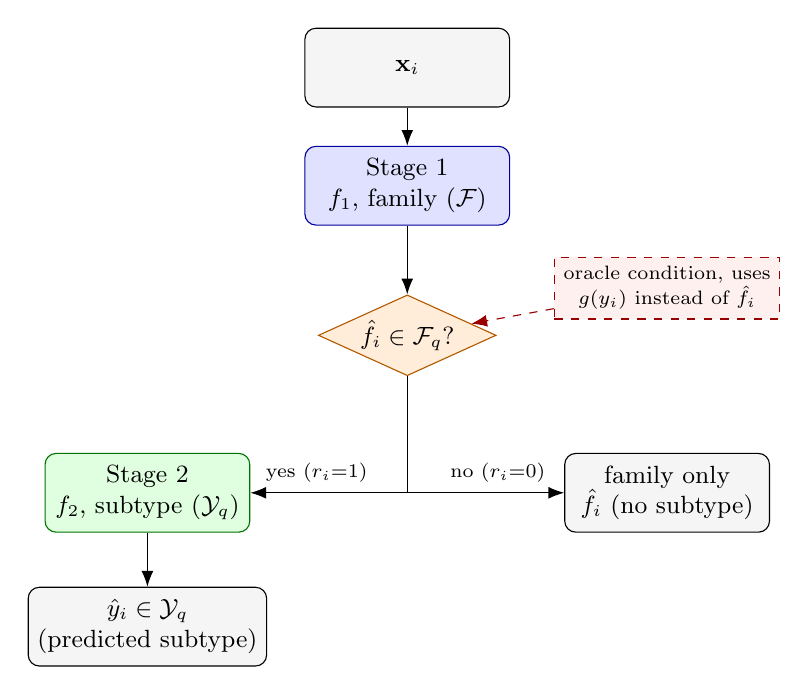
\begin{tikzpicture}[
  every node/.style={font=\small},
  box/.style={draw, rounded corners, align=center, minimum width=2.6cm, minimum height=1.0cm, fill=gray!8},
  stageone/.style={draw=blue!60!black, rounded corners, align=center, minimum width=2.6cm, minimum height=1.0cm, fill=blue!12},
  stagetwo/.style={draw=green!45!black, rounded corners, align=center, minimum width=2.6cm, minimum height=1.0cm, fill=green!12},
  dec/.style={draw=orange!70!black, diamond, aspect=2.2, align=center, inner sep=1pt, font=\small, fill=orange!15},
  oraclebox/.style={draw=red!60!black, dashed, align=center, font=\scriptsize, minimum width=2.8cm, fill=red!6},
  arr/.style={-{Latex[length=2mm,width=1.5mm]}},
]

\node[box] (x1) at (0,7.4) {$\mathbf{x}_i$};
\node[stageone] (f1) at (0,5.9) {Stage 1\\$f_1$, family ($\mathcal{F}$)};
\node[dec] (dec) at (0,4.0) {$\hat{f}_i \in \mathcal{F}_q$?};
\node[stagetwo] (f2) at (-3.3,2.0) {Stage 2\\$f_2$, subtype ($\mathcal{Y}_q$)};
\node[box] (outsub) at (-3.3,0.3) {$\hat{y}_i \in \mathcal{Y}_q$\\(predicted subtype)};
\node[box] (outfam) at (3.3,2.0) {family only\\$\hat{f}_i$ (no subtype)};
\node[oraclebox] (oracle) at (3.3,4.6) {oracle condition, uses\\$g(y_i)$ instead of $\hat{f}_i$};

\draw[arr] (x1) -- (f1);
\draw[arr] (f1) -- (dec);
\draw[arr] (dec) |- (f2);
\node[font=\scriptsize] at (-1.15,2.25) {yes ($r_i{=}1$)};
\draw[arr] (f2) -- (outsub);
\draw[arr] (dec) |- (outfam);
\node[font=\scriptsize] at (1.15,2.25) {no ($r_i{=}0$)};
\draw[dashed, arr, red!60!black] (oracle) -- (dec);

\end{tikzpicture}%
}
\caption{Visualization of the hierarchical detection framework.}
\label{fig:framework}
\end{figure}

Figure~\ref{fig:framework} details the routing process. Stage 1 predicts the
family ($\mathcal{F}$), and Stage 2, shown in green, is activated only when
the prediction belongs to $\mathcal{F}_q$ (PQ or Hybrid). The red dashed box
shows the oracle condition, which replaces the predicted family with the true
family at this decision point. The flat classifier does not use this routing
process. It predicts the 24 classes directly from $\mathbf{x}_i$.

Stage 1 predicts the attack family from the selected feature vector. Its output
determines the routing decision for the second stage in the predicted-routing
cascade, represented by the diamond in Figure~\ref{fig:framework}. Family-level
errors are retained in the final evaluation because an incorrect prediction
can prevent selection of the appropriate subtype classifier.

Stage 2 is trained for the relevant post-quantum and hybrid families and
predicts the subtype associated with the selected family. Its performance is
first measured under oracle routing and then under routing generated by Stage
1, separating the capacity of the specialized model from the effect of errors
in the previous stage.

The flat baseline uses the same predictors, training partitions, model families,
preprocessing, random seeds, and evaluation metrics as the hierarchical
structure, but directly predicts one of the 24 labels without an intermediate
routing decision. It provides the reference for examining the effect of the
additional label structure.

Under predicted routing, each test record passes through Stage 1 and is sent to
Stage 2 according to the predicted family rather than the true family. The
final prediction combines the family decision with the subtype prediction of
the specialized model. Records sent to an incorrect family are counted as
cascade errors and are not corrected using the true label. This procedure
evaluates the behavior of the sequential detector in contrast to the isolated
oracle condition in Figure~\ref{fig:framework}.

The four components described above, namely Stage 1, Stage 2, the flat
baseline, and the distinction between oracle and predicted routing, are trained
and evaluated under the same leakage-audit protocol, identity-based grouped split,
and separation of real and synthetic traces. The next section details the
models, hyperparameters, and computational environment used to instantiate
them.
\section{Implementation and Experimental Setup}
\label{sec:models}
This section details how the detection framework described above was
implemented. It specifies the supervised algorithms and their hyperparameters,
the training and preprocessing procedures, the reported metrics, and the
computational environment used to produce the results below.

The classifiers $f_{\mathrm{flat}}$, $f_1$, and $f_2$ are instantiated with
four supervised algorithms. These are LightGBM, the primary model for the
central comparisons \cite{ke2017lightgbm}, logistic regression, random forest,
and a fully connected neural network or MLP. All models use the same random
seed ($\mathrm{seed}=42$) and run entirely on the CPU. The selected
hyperparameters are shown in Table~\ref{tab:hyperparams}. Balanced sample
weights provided by the scikit-learn package \cite{pedregosa2011scikit} are
used when fitting LightGBM, logistic regression, and random forest. The
\texttt{MLPClassifier} provided by scikit-learn does not accept sample weights
in \texttt{.fit()} and is therefore trained without class weighting. This is a
documented model constraint rather than a design choice.

\begin{table}[!t]
\caption{Model hyperparameters (all models, seed = 42)}
\label{tab:hyperparams}
\centering
\begin{tabular}{ll}
\toprule
Model & Key hyperparameters \\
\midrule
LightGBM & n\_estimators = 200 \\
Logistic regression & max\_iter = 200 \\
Random forest & n\_estimators = 200 \\
MLP & hidden\_layer\_sizes = (64, 32), max\_iter = 300 \\
\bottomrule
\end{tabular}
\end{table}

Numerical and categorical attributes are preprocessed separately. Numerical
attributes receive median imputation followed by standardization with zero
mean and unit variance. Categorical attributes receive constant filling with
\texttt{"missing"} followed by one-hot encoding, with unseen categories
ignored during inference. All models and compared conditions use the same
training, validation, and test split, approximately 70\%, 15\%, and 15\%,
stratified by label and grouped by feature identity so that no duplicate
pattern crosses partitions. The primary seed is 42, and LightGBM stability is
checked with two additional seeds, 123 and 2024.

The reported metrics are macro-F1, which is the primary metric defined above,
accuracy, and the complete confusion matrix at both the family and subtype
levels. Per-class precision and recall are also reported for subtype
classification. Routing precision and recall are additionally reported for the
cascade under predicted routing. All metrics are computed on the test partition and
never on training or validation data.

All experiments run entirely on the CPU without GPU use, with Python 3.11.0
on Windows on a machine with an Intel Core i5-1135G7 processor
(11th generation, 2.40\,GHz) and 32\,GB of RAM. The software packages are
pandas 3.0.3, pyarrow 25.0.0, h5py 3.16.0, scikit-learn 1.6.1, lightgbm 4.6.0,
and numpy 1.26.4. As a computational reference, LightGBM Stage 1 training on
3,571,400 training records from the original release takes 287.5 seconds, and
Stage 2 training on the PQ/Hybrid subset takes 219.3 seconds. In the extended
release, the corresponding times are 230.9 and 243.0 seconds. The grouped
split itself, dominated by hashing predictor attributes for five million
records, takes 179.3 seconds in the original release and 89.3 seconds in the
extended release. The code, parameters, seeds, and 42 automated pytest checks
used to audit the pipeline are versioned with the study to support independent
reproduction.

These four elements, namely the models and hyperparameters, the training and
preprocessing procedure, the reported metrics, and the computational
environment, are applied identically to all conditions compared in the next
section. These conditions include Stage 1, Stage 2 under oracle and predicted
routing, and the flat baseline in both data releases.

\section{Experimental Results}
This section reports family and subtype detection performance for the four
compared algorithms, the central comparison between the hierarchical
architecture and the flat baseline, the difference between the original and
extended releases, result stability across real and synthetic traces and
random seeds, and the computational cost of each stage. All values follow the
data protocol and training procedure described above.

The four algorithms are analyzed separately at the family level and at the
subtype level under oracle routing. At the family level, LightGBM is not the
highest-scoring individual model. MLP has the highest value in the original
release, whereas random forest has the highest value in the extended release
by a small margin. LightGBM was nevertheless defined a priori as the primary
model for the central comparisons, before the individual model results were
reported. At the subtype level under oracle routing, the four models have
similar values in both corpora, suggesting that PQ and Hybrid subtype
difficulty is not determined by algorithm choice alone.
\begin{table}[!t]
\caption{Macro-F1 by model on the test partition, for attack-family
detection (Stage 1) and exact-subtype detection under oracle routing
(Stage 2).
Orig.\ = original release, Ext.\ = extended release. Best model per column in
bold; the last two rows are trivial predictors, not trained models}
\label{tab:stage_by_model}
\centering
\begin{tabular}{lrrrr}
\toprule
 & \multicolumn{2}{c}{Stage 1 (family)} & \multicolumn{2}{c}{Stage 2 (subtype, oracle)} \\
Model & Orig. & Ext. & Orig. & Ext. \\
\midrule
LightGBM & 0.5864 & 0.8796 & \textbf{0.4233} & \textbf{0.4289} \\
Logistic regression & 0.4806 & 0.8700 & 0.4169 & 0.4220 \\
Random forest & 0.5992 & \textbf{0.8801} & 0.4153 & 0.4175 \\
MLP & \textbf{0.6056} & 0.8561 & 0.4133 & 0.4201 \\
\midrule
Majority class & 0.1871 & 0.1876 & 0.0078 & 0.0075 \\
Stratified random & 0.2505 & 0.2500 & 0.0525 & 0.0529 \\
\bottomrule
\end{tabular}
\end{table}


\begin{figure}[!t]
\centering
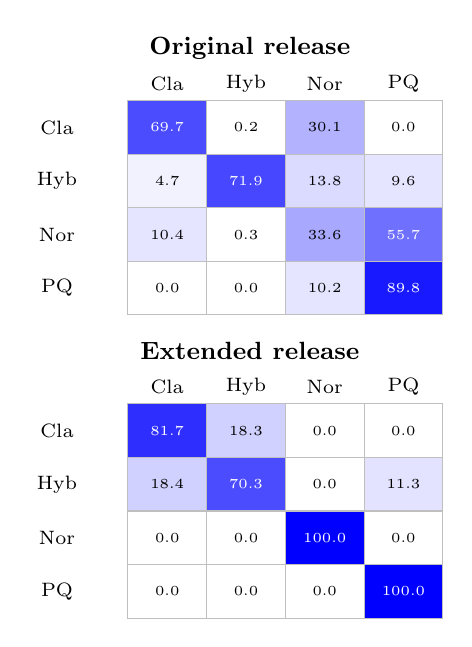
\begin{tikzpicture}[
  every node/.style={font=\tiny},
  cell/.style={draw=gray!50, minimum width=1.0cm, minimum height=0.68cm, align=center},
  lbl/.style={font=\scriptsize},
]
\node[font=\small\bfseries] at (2.45,1.35) {Original release};
\node[lbl] at (1.4,0.90) {Cla};
\node[lbl] at (2.4,0.90) {Hyb};
\node[lbl] at (3.4,0.90) {Nor};
\node[lbl] at (4.4,0.90) {PQ};
\node[lbl] at (0.0,0.34) {Cla};
\node[cell, fill=blue!70, text=white] at (1.4,0.34) {69.7};
\node[cell, fill=blue!0] at (2.4,0.34) {0.2};
\node[cell, fill=blue!30] at (3.4,0.34) {30.1};
\node[cell, fill=blue!0] at (4.4,0.34) {0.0};
\node[lbl] at (0.0,-0.34) {Hyb};
\node[cell, fill=blue!5] at (1.4,-0.34) {4.7};
\node[cell, fill=blue!72, text=white] at (2.4,-0.34) {71.9};
\node[cell, fill=blue!14] at (3.4,-0.34) {13.8};
\node[cell, fill=blue!10] at (4.4,-0.34) {9.6};
\node[lbl] at (0.0,-1.02) {Nor};
\node[cell, fill=blue!10] at (1.4,-1.02) {10.4};
\node[cell, fill=blue!0] at (2.4,-1.02) {0.3};
\node[cell, fill=blue!34] at (3.4,-1.02) {33.6};
\node[cell, fill=blue!56, text=white] at (4.4,-1.02) {55.7};
\node[lbl] at (0.0,-1.70) {PQ};
\node[cell, fill=blue!0] at (1.4,-1.70) {0.0};
\node[cell, fill=blue!0] at (2.4,-1.70) {0.0};
\node[cell, fill=blue!10] at (3.4,-1.70) {10.2};
\node[cell, fill=blue!90, text=white] at (4.4,-1.70) {89.8};
\node[font=\small\bfseries] at (2.45,-2.5) {Extended release};
\node[lbl] at (1.4,-2.95) {Cla};
\node[lbl] at (2.4,-2.95) {Hyb};
\node[lbl] at (3.4,-2.95) {Nor};
\node[lbl] at (4.4,-2.95) {PQ};
\node[lbl] at (0.0,-3.51) {Cla};
\node[cell, fill=blue!82, text=white] at (1.4,-3.51) {81.7};
\node[cell, fill=blue!18] at (2.4,-3.51) {18.3};
\node[cell, fill=blue!0] at (3.4,-3.51) {0.0};
\node[cell, fill=blue!0] at (4.4,-3.51) {0.0};
\node[lbl] at (0.0,-4.19) {Hyb};
\node[cell, fill=blue!18] at (1.4,-4.19) {18.4};
\node[cell, fill=blue!70, text=white] at (2.4,-4.19) {70.3};
\node[cell, fill=blue!0] at (3.4,-4.19) {0.0};
\node[cell, fill=blue!11] at (4.4,-4.19) {11.3};
\node[lbl] at (0.0,-4.87) {Nor};
\node[cell, fill=blue!0] at (1.4,-4.87) {0.0};
\node[cell, fill=blue!0] at (2.4,-4.87) {0.0};
\node[cell, fill=blue!100, text=white] at (3.4,-4.87) {100.0};
\node[cell, fill=blue!0] at (4.4,-4.87) {0.0};
\node[lbl] at (0.0,-5.55) {PQ};
\node[cell, fill=blue!0] at (1.4,-5.55) {0.0};
\node[cell, fill=blue!0] at (2.4,-5.55) {0.0};
\node[cell, fill=blue!0] at (3.4,-5.55) {0.0};
\node[cell, fill=blue!100, text=white] at (4.4,-5.55) {100.0};
\end{tikzpicture}
\caption{Stage 1 confusion matrices on the test partition (LightGBM,
row-normalized \%). Rows are the true family, columns the predicted family.
Cla = Classical, Hyb = Hybrid, Nor = Normal, PQ = Post-Quantum.}
\label{fig:confusion_stage1}
\end{figure}


Figure~\ref{fig:confusion_stage1} details this difference by family. In the
original release, 55.7\% of records whose true family is Normal are classified
as Post-Quantum, while only 33.6\% remain in the Normal class. This majority
error directs a substantial portion of normal traffic to Stage 2, which was
not trained to produce normal labels. In the extended release, Normal and
Post-Quantum have 100.0\% separation in the matrix, while residual confusion
is concentrated between Classical and Hybrid. The family-level structure is
therefore substantially clearer in the extended release.

LightGBM has a higher family-level value than the flat baseline in both corpora
and also has a higher subtype-level value when Stage 2 receives the true
family. When Stage 2 uses routing produced by Stage 1, accumulated errors
change this relation and the flat baseline has the higher macro-F1 in both
corpora. This result shows that the interpretation of the hierarchy depends on
routing quality and cannot be derived from ideal evaluation alone. The complete
comparison between the 24-class flat classifier and the two-level hierarchical
architecture is presented in Table~\ref{tab:flat_vs_hier}.

\begin{table}[!t]
\caption{Flat baseline versus hierarchical architecture on the test partition
(LightGBM, macro-F1). Oracle supplies the true family; Predicted scores only
the rows Stage 1 routed; End-to-end scores every truly PQ/Hybrid row, counting
those the cascade never routed as errors. Better value of each pair in bold}
\label{tab:flat_vs_hier}
\centering
\small
\begin{tabular}{lllrr}
\toprule
Level & Model & Condition & Original & Extended \\
\midrule
Family ($\mathcal{F}$) & $f_1$ (Stage 1) &  & \textbf{0.5864} & \textbf{0.8796} \\
Family ($\mathcal{F}$) & $f_{\mathrm{flat}}$ &  & 0.4962 & 0.8726 \\
\midrule
Subtype ($\mathcal{Y}_q$) & $f_2$ (Stage 2) & Oracle & \textbf{0.4233} & \textbf{0.4289} \\
Subtype ($\mathcal{Y}_q$) & $f_{\mathrm{flat}}$ & Oracle & 0.3757 & 0.4130 \\
\midrule
Subtype ($\mathcal{Y}_q$) & $f_2$ (cascade) & Predicted & 0.3236 & 0.3753 \\
Subtype ($\mathcal{Y}_q$) & $f_{\mathrm{flat}}$ & Predicted & \textbf{0.3479} & \textbf{0.3903} \\
\midrule
Subtype ($\mathcal{Y}_q$) & $f_2$ (cascade) & End-to-end & 0.3695 & 0.4112 \\
Subtype ($\mathcal{Y}_q$) & $f_{\mathrm{flat}}$ & End-to-end & \textbf{0.3757} & \textbf{0.4130} \\
\bottomrule
\end{tabular}
\end{table}


Stage 1 routing quality, measured by routing precision and recall in
Table~\ref{tab:multiseed}, explains part of the difference between oracle and
predicted-routing conditions. It is substantially higher in the extended release, which is
consistent with the confusion matrix in Figure~\ref{fig:confusion_stage1}. At
the family level, the hierarchical and flat approaches have different values
across both corpora. At the subtype level, the Stage 2 value exceeds the flat
value only under oracle routing. Under predicted routing, the flat value is
higher in both corpora.

Across the comparisons reported in this section, the extended release has
higher values than the original release at the family level
(Table~\ref{tab:stage_by_model}), at the subtype level under oracle and predicted
routing (Table~\ref{tab:flat_vs_hier}), and in multi-seed robustness
(Table~\ref{tab:multiseed}). The relative difference is larger at the family
level than at the subtype level, which is consistent with the structural
difference in the completeness of sparse cryptographic attributes between the
two releases.

In the original release, records with real traces have higher Stage 1 macro-F1
values than synthetic traces with LightGBM, while in the extended release the
synthetic traces reach a slightly higher value. This is an observed association
rather than evidence that either trace type is intrinsically more difficult to
classify, because the difference may arise from how synthetic traces are
generated. The values for each release are shown in
Table~\ref{tab:real_synthetic}, with the higher value in each pair in bold.

\begin{table}[!t]
\caption{Stage 1 on the test partition (LightGBM, family level), real
versus synthetic traces. Higher value of each pair in bold}
\label{tab:real_synthetic}
\centering
\begin{tabular}{llrr}
\toprule
Release & Trace & Macro-F1 & Accuracy \\
\midrule
Original & Real & \textbf{0.6281} & \textbf{0.5633} \\
Original & Synthetic & 0.5819 & 0.5149 \\
Extended & Real & 0.8646 & 0.9376 \\
Extended & Synthetic & \textbf{0.8812} & \textbf{0.9459} \\
\bottomrule
\end{tabular}
\end{table}


The main finding remains stable across the three seeds. The flat value is
higher than the Stage 2 value under predicted routing for all seeds and in both
corpora, while the change between oracle and predicted routing at the subtype level
also persists. Stage 1 routing precision remains stable across seeds,
indicating that the difference in routing quality between releases is not an
artifact of a single data split. Means and population standard deviations for
the central metrics are reported in Table~\ref{tab:multiseed}.

The end-to-end condition does not share this stability. In the original
release the flat classifier leads in all three seeds, but in the extended
release one seed reverses the ordering, so the end-to-end comparison is
treated here as inconclusive for that release. This is consistent with its
bootstrap interval, which is the only one of the four that approaches zero.

\begin{table}[!t]
\caption{Multi-seed robustness on the test partition (LightGBM, mean $\pm$
population standard deviation across seeds 42, 123, 2024; macro-F1
unless noted)}
\label{tab:multiseed}
\centering
\small
\begin{tabular}{lrr}
\toprule
Metric & Original & Extended \\
\midrule
Stage 1 & 0.5865 $\pm$ 0.0023 & 0.8787 $\pm$ 0.0059 \\
Stage 2, oracle & 0.4200 $\pm$ 0.0025 & 0.4306 $\pm$ 0.0043 \\
Stage 2, predicted routing & 0.3168 $\pm$ 0.0099 & 0.3772 $\pm$ 0.0035 \\
Flat, predicted routing & 0.3314 $\pm$ 0.0141 & 0.3935 $\pm$ 0.0026 \\
Stage 2, end-to-end & 0.3666 $\pm$ 0.0021 & 0.4134 $\pm$ 0.0034 \\
Flat, end-to-end & 0.3792 $\pm$ 0.0033 & 0.4140 $\pm$ 0.0010 \\
Routing precision & 0.4361 $\pm$ 0.0053 & 0.9404 $\pm$ 0.0033 \\
Routing recall & 0.8619 $\pm$ 0.0022 & 0.9234 $\pm$ 0.0020 \\
\bottomrule
\end{tabular}
\end{table}


Because the central claim is a difference of a few hundredths of macro-F1
between two classifiers scored on identical rows, it is reported with an
interval rather than as a point estimate. Resampling those rows with
replacement and recomputing both scores on each resample cancels the shared
sampling noise and leaves the disagreement between the two models.
Table~\ref{tab:bootstrap} reports the result. Under predicted routing the
interval excludes zero in both releases by a clear margin. Under end-to-end
scoring it excludes zero in the original release, while in the extended
release the interval reaches close to zero, which together with the seed
variation above is why that particular comparison is not claimed.

\begin{table*}[!t]
\caption{Paired bootstrap of the flat-minus-cascade macro-F1 difference
(LightGBM, 1,000 resamples of the same rows, 95\% percentile
interval). A positive value favors the flat classifier; an interval excluding
zero separates the two architectures}
\label{tab:bootstrap}
\centering
\small
\begin{tabular}{lcc}
\toprule
Condition & Original & Extended \\
\midrule
Predicted routing & $+0.0243$ $[+0.0199, +0.0286]$ & $+0.0151$ $[+0.0134, +0.0168]$ \\
End-to-end & $+0.0062$ $[+0.0048, +0.0076]$ & $+0.0018$ $[+0.0001, +0.0034]$ \\
\bottomrule
\end{tabular}
\end{table*}


Finally, the effect of the splitting rule itself is isolated in
Table~\ref{tab:split_ablation}. Data, model, hyperparameters, and scale are
held fixed, and only the partitioning changes, from grouping by feature
identity to the plain stratified random split used by the original benchmark.
Under random splitting essentially every evaluation row has an exact
predictor-value twin sitting in the training partition, and macro-F1 rises to
near-perfect values across all three tasks. The gap between the two rows of
each pair is therefore attributable to duplicate patterns crossing the
train/test boundary rather than to any difference in model or data, which
places the near-perfect scores reported under random splitting in
Table~\ref{tab:external_baseline} in context.

\begin{table*}[!t]
\caption{Split ablation (LightGBM, identical data, model, and scale; only the
splitting rule changes). Twinned is the share of test rows holding an exact
predictor-value twin in the training partition}
\label{tab:split_ablation}
\centering
\small
\begin{tabular}{llrrr}
\toprule
Release & Split & Twinned & Stage 1 & Flat 24-class \\
\midrule
Original & Grouped by feature identity & 0.0\% & 0.5864 & 0.3815 \\
Original & Plain random & 100.0\% & 0.6773 & 0.6795 \\
Extended & Grouped by feature identity & 0.0\% & 0.8796 & 0.4673 \\
Extended & Plain random & 100.0\% & 0.9809 & 0.9947 \\
\bottomrule
\end{tabular}
\end{table*}


Computational cost varies across stages because the flat baseline is trained on
all classes and training records, whereas Stage 2 uses only the PQ/Hybrid
subset. Stage 1 and the flat baseline also reflect the cost of training four
models on the same machine described above. The observed time therefore
depends on both the architecture and the amount of data processed at each
stage. Complete times by stage and release are shown in Table~\ref{tab:runtime}.

\begin{table}[!t]
\caption{Training wall-clock time, four-model run (minutes)}
\label{tab:runtime}
\centering
\begin{tabular}{lrr}
\toprule
Stage & Original & Extended \\
\midrule
Grouped split & 3.0 & 1.5 \\
Stage 1 (4 models) & 63.4 & 105.0 \\
Stage 2 (4 models) & 31.1 & 41.4 \\
Flat baseline (4 models) & 77.6 & 130.7 \\
\bottomrule
\end{tabular}
\end{table}

Taken together, the results support two central conclusions. The hierarchical
and flat approaches show different behavior at the family level, while at the
subtype level the relationship changes when routing moves from oracle
information to predictions produced by Stage 1. Both conclusions hold in both
corpora and, for LightGBM, across the three seeds; the remaining three
algorithms were evaluated at the primary split only, so their ordering is not
claimed to be seed-independent. The next section discusses these findings for
intelligent transportation detection architectures.

\section{Discussion}
The experiments compared family- and subtype-level detection for four
algorithms, evaluated the hierarchical architecture and flat baseline under
oracle and predicted routing, and examined both data releases, trace types,
and three random seeds. The Stage 1 confusion matrix and training times
complement the performance comparison by describing routing behavior and
computational cost.

\subsection{Answer to the Research Question}
At the family level, Stage 1 exceeds the flat baseline in both releases,
with macro-F1 values of 0.5864 versus 0.4962 in the original release and
0.8796 versus 0.8726 in the extended release. At the subtype level, Stage 2
also exceeds the flat classifier under oracle routing, reaching 0.4233 versus
0.3757 and 0.4289 versus 0.4130 in the original and extended releases,
respectively. Under predicted routing, the relation reverses and the flat
classifier reaches 0.3479 versus 0.3236 and 0.3903 versus 0.3753. The
three-seed analysis preserves this relation in both releases, establishing the
reversal as the central empirical finding.

\subsection{Implications for Intelligent Transportation Systems}
In a vehicular security architecture, an intrusion detector operates on messages that may represent normal cooperative traffic or various attack families. The family-level decision organizes message forwarding and determines which specialized analysis is executed next. The observed Stage 1 values show that this stage has its own behavior and should be evaluated separately from subtype classification. This separation matters because a family decision is not only an intermediate model output; it also governs the operational analysis path of the record.

These findings bear on how detection is organized across On-Board Units (OBUs), Roadside Units (RSUs), and Mobile Edge Computing (MEC) servers. The considerations below follow from the detection results reported here; this study measures training cost on a general-purpose CPU and does not measure inference latency, memory, or energy on vehicular hardware, so they are design implications rather than deployment measurements.
\begin{itemize}
    \item \textbf{Routing risk is an architectural cost, not only a metric.} A single-pass flat classifier has no forwarding decision that can fail, so it cannot lose a record to misrouting. The cascade can. In the original release a substantial share of the records reaching Stage 2 do not belong to its label space at all, while some genuine PQC-related attacks never arrive. For a safety-relevant detector this is a qualitatively different failure mode from an ordinary misclassification, because the record leaves the analysis path entirely.
    \item \textbf{Where a hierarchy remains attractive.} If a hierarchical architecture is chosen, the family stage is the natural place to partition work, with a lightweight Stage 1 triaging traffic locally on the OBU or RSU and suspected PQC-related payloads offloaded to MEC or Traffic Management Center infrastructure for subtype classification. Our results indicate that such a design should gate that offload on calibrated confidence rather than on the arg-max family decision, since it is precisely the unconditional forwarding of the arg-max decision that produces the reversal reported here. Confidence-gated routing was not evaluated in this study and remains an open direction.
\end{itemize}

This distinction directly affects the system-level result. When forwarding is incorrect, a record may not reach the subtype classifier associated with its family, and the error becomes part of the final cascade decision. Joint analysis at the family and subtype levels therefore provides separate information about the initial decision, second-stage specialization, and error propagation between stages.

\subsection{Interpretation of Routing Errors}
The difference between the values obtained under oracle and predicted routing (Table~\ref{tab:flat_vs_hier}) quantifies the portion of the Stage 2 result associated with the Stage 1 decision rather than with the specialized classifier itself. This distance is larger in the original release than in the extended release, following the observed change in routing quality between releases (Table~\ref{tab:multiseed}).

The Stage 1 confusion matrix (Figure~\ref{fig:confusion_stage1}) explains this difference in terms of the routing false positives and false negatives defined above ($r_i=1, r_i^{\star}=0$ and $r_i=0, r_i^{\star}=1$, respectively). In the original release, confusion between Normal and Post-Quantum is the main source of false-positive routing. Because Normal is the most frequent family (Table~\ref{tab:family_dist}), the error sends a substantial number of normal records to Stage 2, which was not trained to output the Normal class. In the extended release, the separation between Normal and Post-Quantum is nearly complete, while residual confusion between Classical and Hybrid still produces routing errors but affects a smaller fraction of records because these two families are less frequent than Normal. The pattern shows that routing quality depends on both family separability in the available attributes and the relative frequency of each family in the traffic.

This result also clarifies the difference between evaluating Stage 2 capacity and evaluating the complete cascade. Oracle routing preserves the true family and isolates subtype classification, whereas predicted routing includes forwarding errors and measures the sequence of decisions used by the detector. The distance between these conditions measures how much the initial decision changes the final result.

\subsection{Practical Scope, Limitations, and Threats to Validity}
The experimental framework established in this study provides a reproducible benchmark across 5~million records that isolates architectural effects before embarking on costly hardware prototyping. The protocol controls exact-duplicate leakage, which is the dominant form in this dataset, but it does not establish that the data are leakage-free in every sense, as the bullets below make explicit. To contextualize the empirical findings for practical ITS deployments, several methodological characteristics and scope boundaries should be noted.

\begin{itemize}
    \item \textbf{Dataset-based benchmarking versus physical testbeds.} The analysis relies on the PQ-V2X dataset, which provides extensive tabular coverage of mobility, channel, and post-quantum cryptographic parameters across real and synthetic traces. While this large-scale dataset enables controlled, multi-seed comparative benchmarking, it remains an offline representation. Future work should build directly on these architectural insights by validating flat and hierarchical detectors on hardware-in-the-loop (HIL) vehicular testbeds, evaluating end-to-end processing latencies, memory constraints, and energy consumption on embedded automotive microcontrollers and OBUs.
    \item \textbf{Temporal traffic dynamics and streaming evaluations.} The supervised classification conducted here operates on discrete tabular records without tracking continuous temporal packet streams or vehicle-to-vehicle trajectory sequences. In operational V2X networks, periodic message broadcasts (such as 10~Hz BSM/CAM streams) introduce temporal correlations. Evaluating streaming detectors that incorporate temporal windowing or sequential state tracking represents a natural extension.
    \item \textbf{Duplicate grouping versus trajectory tracking.} To prevent optimistic performance estimates caused by exact-duplicate leakage, records are grouped by a deterministic feature hash. This approach effectively controls for identical feature patterns across partitions. However, consecutive messages generated during a single vehicle trip may exhibit slight feature drift (e.g., gradually changing GPS coordinates or timestamps), forming near-duplicates. Future datasets with standardized, granular trajectory identifiers will enable even stricter trip-level grouping.
    \item \textbf{Synthetic trace separability.} The extended release exhibits near-perfect Stage~1 family separability for Normal and Post-Quantum traffic (Figure~\ref{fig:confusion_stage1}), with Normal reaching exactly 100\% row-normalized accuracy and zero misclassified records. The leakage audit in Table~\ref{tab:leakage_audit} tests individual candidate columns against the binary attack target and therefore cannot rule out multivariate leakage, in which a combination of columns that each fall below the AUC threshold jointly separates a class almost perfectly. Because the original release shares the same label taxonomy yet shows no such separability, it is at least as plausible that this reflects an artifact of how the extended release's records were generated as that it reflects a genuinely easier detection task. Family-level results on the extended release should accordingly be read as an upper bound obtained under this dataset's specific generation process, not as an estimate of achievable performance on real, more heterogeneous V2X traffic.
    \item \textbf{Scope of the multi-seed analysis.} The four-algorithm comparison is complete at the primary split, but the repeated-seed robustness analysis covers LightGBM only. The relative ordering of logistic regression, random forest, and MLP should therefore be read as evidence from a single split rather than as a claim of seed-independent superiority. Extending multi-seed evaluation to all four algorithms is a useful follow-up; it is not required to interpret the primary LightGBM comparison, which is the basis of every claim made here.
    \item \textbf{Untuned model capacity.} No hyperparameter search was performed. Every algorithm runs at a fixed, documented configuration so that the flat and hierarchical arms receive an identical budget, which is what makes the architectural comparison interpretable. The consequence is that the absolute values are not the best attainable for any algorithm, and the comparison establishes an ordering at one capacity point rather than across the capacity range. Convergence status is reported with the results so that a weak baseline can be distinguished from an under-trained one.
\end{itemize}

\section{Conclusion}

This study presented a controlled experimental comparison between a hierarchical detector and a 24-class flat classifier for PQC-related attack detection in connected transportation systems. By employing a duplicate-aware grouped splitting protocol, family- and subtype-level metrics, Stage~1 predicted routing, two PQ-V2X data releases, real and synthetic traces, a four-algorithm comparison at the primary split, and multi-seed validation of the primary LightGBM model, the evaluation provides a reproducible baseline that avoids the data-leakage pitfalls of naive random splits.

The findings establish that while hierarchical classification improves coarse family-level identification and outperforms the flat baseline under idealized oracle routing, this advantage reverses once operational Stage~1 predictions govern the cascade, where the flat classifier achieves higher subtype macro-F1 in both data releases and across all random seeds. This reversal demonstrates that isolated component capacity does not guarantee cascade superiority in operational pipelines.

Future work will extend these architectural findings to physical vehicular testbeds and Hardware-in-the-Loop (HIL) environments, measuring real-time inference latency, energy overhead, and memory footprints on embedded automotive OBUs and edge RSUs. Additional directions include evaluating continuous temporal traffic streams, cross-dataset validation under diverse mobility scenarios, and adaptive confidence-gated routing strategies for distributed ITS security.

\section*{Data Availability}

The PQ-V2X dataset analyzed in this study was created and is distributed by
Abdel Hakeem and Kim \cite{105018710169}; it is not redistributed here. All
code, evaluation protocol, hyperparameters, random seeds, automated tests, run
logs, and the complete result files behind every table in this paper are
openly archived under DOI \texttt{10.5281/zenodo.22965246}. Reported metrics are
computed on a held-out test partition; the validation partition is never read,
and each archived result file records the partition that produced it.

\bibliographystyle{IEEEtran}
\bibliography{references}


\begin{IEEEbiographynophoto}{Marcos Batista Figueredo}
holds the M.Sc. and Ph.D. degrees in Computational Modeling and Industrial
Technology and has over 20 years of experience in higher education. He works
in mathematical modeling, computer vision, pattern recognition, and renewable
energy. He has coordinated the Master's Program in Modeling and Simulation of
Biosystems at Universidade do Estado da Bahia and contributed to research
projects involving renewable energy systems, visual computing, and applied
mathematical models.
\end{IEEEbiographynophoto}

\begin{IEEEbiographynophoto}{Lizandra Santos Morais}
is a dental surgeon (CRO-BA 31407) and an M.Sc. student in Biosystems Modeling and Simulation at Universidade do Estado da Bahia. She holds a degree in Dentistry from FATEC-BA and served as Project Director of the Academic League of Oral and Maxillofacial Surgery and Traumatology (2024--2025). Her research focuses on regenerative medicine, digital health, and computational modeling.
\end{IEEEbiographynophoto}


\begin{IEEEbiographynophoto}{Thiago Barros Murari}
is the Coordinator of the Graduate Program in Industrial Management and
Technology and a faculty member of the Graduate Program in Computational
Modeling and Industrial Technology at SENAI CIMATEC University Center. His
research interests include innovation, Industry 4.0, digital transformation,
mobility, and complex systems. He is also co-leader of the CNPq Research Group
on Virtual and Augmented Reality for Innovation in Industry.
\end{IEEEbiographynophoto}
% Not included, pending confirmation: Deputy Director of the Brazilian Center
% for Applied Research in Artificial Intelligence of the MCTI.

\begin{IEEEbiographynophoto}{Alexandre do Nascimento Silva}
received the Ph.D. degree in Computational Modeling and Industrial Technology
from SENAI CIMATEC University Center. He is a professor at Universidade
Estadual de Santa Cruz and at the Master's Program in Modeling and Simulation
of Biosystems at Universidade do Estado da Bahia. His research focuses on
computational modeling and neuronal biosystem modeling. He has contributed to
projects on neural network mapping, learning capacity, and neurobiological
process representation, and has authored over 20 scientific publications.
\end{IEEEbiographynophoto}

\begin{IEEEbiographynophoto}{Neraldo de Ara\'{u}jo Fontoura}
is a mathematics professor and an M.Sc. student in Biosystems Modeling and Simulation, with experience in mathematics, particularly applied mathematics.
\end{IEEEbiographynophoto}

\begin{IEEEbiographynophoto}{Jos\'{e} Roberto de Ara\'{u}jo Fontoura}
holds a Ph.D. degree in Knowledge Diffusion, a Master's degree in Accounting,
and degrees in Accounting and Systems Analysis. His work focuses on
accounting, information management, and the intersection between
organizational processes and computational systems.
\end{IEEEbiographynophoto}

\begin{IEEEbiographynophoto}{Matheus Bahia Silva}
holds a degree in Information Systems from Universidade do Estado da Bahia (2023) and is currently an M.Sc. student in Biosystems Modeling and Simulation at the same institution. He has experience in computer science, particularly computing systems.
\end{IEEEbiographynophoto}

\begin{IEEEbiographynophoto}{Leandro Brito Santos}
holds the M.Sc. and Ph.D. degrees in Computational Modeling and Industrial
Technology and a B.Sc. degree in Information Systems. He is a Data Scientist
Researcher at the Data Science BR Network. He has over 14 years of experience
working with data center systems, information security, and cloud monitoring.
His research interests include software engineering, data science, IoT
systems, maker technologies, and complex systems.
\end{IEEEbiographynophoto}



\begin{IEEEbiographynophoto}{Ta\'{i}s Souza de Andrade Soares}
holds degrees in Information Systems (Est\'{a}cio FIB, 2009) and Mathematics (Famart, 2022), with specializations in Automation, Control and Robotics (SENAI CIMATEC, 2016) and Educational Technologies (UNIAENE, 2025). She is currently an M.Sc. student in Biosystems Modeling and Simulation at Universidade do Estado da Bahia and a vocational education teacher in Bahia. Has professional experience in systems development, programming, databases, and educational robotics. Her research interests include artificial intelligence, mathematical modeling, data science, fuzzy systems, and energy recovery.
\end{IEEEbiographynophoto}


\begin{IEEEbiographynophoto}{Aline de Lurdes Zuliani Lunkes}
received the degree in Mathematics from the Federal University of Santa Maria (UFSM), Brazil, in 2015, the M.Sc. degree in Computational Modeling from the Federal University of Rio Grande (FURG), Brazil, in 2018, and the Ph.D. degree in Computational Modeling from the National Laboratory for Scientific Computing (LNCC), Brazil, in 2023. She is currently a professor at Universidade Federal do Pampa. Her research interests include computational modeling, artificial intelligence, inverse problems, numerical methods, and scientific computing.
\end{IEEEbiographynophoto}



\begin{IEEEbiographynophoto}{Roberto Luiz Souza Monteiro}
holds a postdoctoral degree in Computational Modeling and Industrial
Technology, a Ph.D. degree in Knowledge Diffusion, and master's and bachelor's
degrees in computational and information systems. He is a professor at
Universidade do Estado da Bahia and at SENAI CIMATEC University Center. His
work focuses on informatics and society, complex systems, formal languages,
and applied computational modeling. His research interests include compiler
design, embedded systems, social network analysis, and artificial
intelligence.
\end{IEEEbiographynophoto}

\end{document}
